%%%%%%%%%%%%%%%%%%%%%%%%%%%%%%%%%%%%%%%%%%%%%%%%%%%%%%%%%%%%%%%%%%%%%%%%%%%%%%%%
%2345678901234567890123456789012345678901234567890123456789012345678901234567890
%        1         2         3         4         5         6         7         8

\documentclass[letterpaper, 10 pt, conference]{ieeeconf}  % Comment this line out
                                                          % if you need a4paper
%\documentclass[a4paper, 10pt, conference]{ieeeconf}      % Use this line for a4
                                                          % paper

\IEEEoverridecommandlockouts                              % This command is only
                                                          % needed if you want to
                                                          % use the \thanks command
\overrideIEEEmargins
% See the \addtolength command later in the file to balance the column lengths
% on the last page of the document



% The following packages can be found on http:\\www.ctan.org
\usepackage{graphics} % for pdf, bitmapped graphics files
%\usepackage{epsfig} % for postscript graphics files
%\usepackage{mathptmx} % assumes new font selection scheme installed
%\usepackage{times} % assumes new font selection scheme installed
%\usepackage{amsmath} % assumes amsmath package installed
%\usepackage{amssymb}  % assumes amsmath package installed
\usepackage{graphicx}
\usepackage{algorithm}
\usepackage{algpseudocode}
\usepackage[final]{pdfpages}
\usepackage{multirow}
\usepackage{subfigure}
















\title{\LARGE \bf
%A comparative Study of Many-Objective Evolutionary Algorithm for the Discovery and Security of Software Architectures 
$F$-NSGAIII: An Improved Many-Objective Optimization Algorithm Determining for Appropriate Software Architecture Considering Maintenance and Security Related Metrics
}

\author{ \parbox{7 in}{\centering Al-Jamil Suvo, Siddhartha Shankar Das, Anindya Iqbal\\        
        Department of Computer Science and Engineering\\
        Bangladesh University of Engineering and Technology\\
        Dhaka-1000, Bangladesh\\
        {\tt\small 1305038.ajs@ugrad.cse.buet.ac.bd, siddhartha047@cse.buet.ac.bd, anindya@cse.buet.ac.bd}} 
}

% \author{ \parbox{3 in}{\centering Al-Jamil Suvo
%         \thanks{*Use the $\backslash$thanks command to put information here}\\
%         Faculty of Electrical Engineering, Mathematics and Computer Science\\
%         University of Twente\\
%         7500 AE Enschede, The Netherlands\\
%         {\tt\small h.kwakernaak@autsubmit.com}}
%         \hspace*{ 0.5 in}
%         \parbox{3 in}{ \centering Pradeep Misra**
%         \thanks{**The footnote marks may be inserted manually}\\
%        Department of Electrical Engineering \\
%         Wright State University\\
%         Dayton, OH 45435, USA\\
%         {\tt\small pmisra@cs.wright.edu}}
% }


\begin{document}



\maketitle
\thispagestyle{empty}
\pagestyle{empty}


%%%%%%%%%%%%%%%%%%%%%%%%%%%%%%%%%%%%%%%%%%%%%%%%%%%%%%%%%%%%%%%%%%%%%%%%%%%%%%%%
\begin{abstract} 
Software architecture design for large applications is a very challenging task since it has to consider many objectives including some conflicting ones. The architecture is required to be efficient and to maintain friendly with modular and reusable components. Recommended security design principles may conflict with such efficient and reusable design. Thus, software architects have to deal with multiple design alternatives that need to be evaluated comprehensively to select the one that best matches the criteria of the specific context. To enable software architects make their decision prudently, Many-objective Evolutionary Algorithms have been used to effectively explore design alternatives on high dimensional objective spaces. In this paper, we have formulated a Many-objective optimization problem using ten maintenance and five security metrics relevant to architectural issues. We have also developed a modified and improved version of the popular Non-dominated Sorting based Algorithm (NSGAIII) using Fuzzy logic, which clearly outperforms other state-of-the-art many-objective optimization algorithms in this context.

\end{abstract}


%%%%%%%%%%%%%%%%%%%%%%%%%%%%%%%%%%%%%%%%%%%%%%%%%%%%%%%%%%%%%%%%%%%%%%%%%%%%%%%%
\section{INTRODUCTION}

%\subsection{Problem}
Designing a large-scale software system is a challenging and complex process. 
The early stage of the software development is very significant to make some high-impact decisions about software architecture. Software architects have to confirm that its architectural skeleton is perfect before the design development process starts. To ensure this software architecture must guarantee some quality and security criteria.
Again, if the architecture becomes complex, it becomes very challenging to for the developers to implement. To overcome this problem, a common way is to split the architecture into different components~\cite{szyperski1999component}. First step of the software architecture is the  identification of  all elements of the architecture like interfaces, classes, and their relation. Each component is composed of UML classes. Those components are the core parts of the software. Each of those components work individually and they communicate each other through some connections. This component-based architecture accelerates rapid development and testing of a software. Smaller components
reduce the search space for finding bugs. Again, only modifications of some components may fulfill requirements of changing during development process . Now these features depend on the modularity of the component. Again components performing some particular tasks  can be used as an element of other system. Reusability of those components can reduce both cost and time of software development. When a software is divided into different independent component there raise a security concern. As the components have modularity and they are only integrated through some relationship, other non-ethical components can set up to make a relationship with one or many components of the software to access or modify information. This security concern depends on the type of the relationship among the component. Some types of relationship are very critical for entire software systems. So those component defined and related each other in software architecture determine the functional and non-functional requirements like modularity, performance, reusability and security. \\

%\subsection{Motivation}
Search-based Software Engineering(SBSE) is introduced for software development in recent years. This search-based technique is an automated system can assist software developer to find the best underlying structure. In most cases, those functional and non-functional requirements of the software are potentially conflicting and  competing each other. SBSE is considers problems that involve finding a suitable balance between those requirements. Now each functional and non-functional requirements can be represented by some aggregating characteristics value of the software. Those characteristics value are evaluated by formulating some metrics for the software. In last SBSE studies some metrics are proposed to represents those requirements like modularity, reusability, performance. We have used 10 metrics from different SBSE studies. We select those metrics which are related those requirements. Increasing the number of those conflicting metrics also improve perfection in selecting optimized solutions.  \\

Software security is a major activity in the software security. From a study it has been found that cost of maintaining software security is very high approximately 60\% to 70\% of total software development and support effect ~\cite{sachitano2004security}.  It is tough to detect  vulnerabilities in the main operational codes, so it should be tracked from the early development process. Mainly two properties of software is important for security- accessibility and interaction. Accessibility is data encapsulation a mechanism to protect information from outer interfaces. And, Interaction is cohesion between two modules. Now taking security concern at early stage of the development may reduce  many software vulnerabilities. Last SBSE studies not not include security in their search-bases problem formulation. So we have included security metrics in our SBSE research. As our research and other metrics are based on component of the software architecture, so we have  focused on the component based security and we have designed component based security metrics.\\

Search Based Optimization algorithms are used to address problems in SBSE for finding solutions with optimized metrics value. In previous research, generic many objective algorithms are used to solve this problem ~\cite{ramirez2015approach}. In our research, we have used more metrics of modularity and reusability and added some security metrics. Search ability of those algorithms severely deteriorated by the increase of the number of the objectives ~\cite{ishibuchi2008evolutionary}.  Here at first approach, we have used NAGAIII~\cite{deb2014evolutionary} algorithms to search solutions of the problem. NSGAIII algorithms is widely used in previous studies on this topics. But NSGAIII has not been incorporated with any domain knowledge. NSGAIII is rather a generic algorithm to solve generalized problems. Incorporating NSGAIII with domain knowledge of software engineering can improve the search performance. So we have modified NSGAIII algorithms. To select most optimized solutions from generated possible solutions of SBSE problem, NSGAIII select randomly from last Pareto-Front. We have replaced that selection precess of NSGAIII by Fuzzy based comparison between the solutions in the last Pareto-Front using half Gaussian function. Fuzzy based comparison performs better in no-dominated solutions. That is why we have achieved some improvement in our proposed Fuzzy based NSGAIII ( \textit{F}-NSGAIII ) over general NAGAIII.  

%Novelty
The novelty of our works can be summarized as follows:

\begin{itemize}
\item we have adapted 10 different performance, modularity, and maintenance metrics 
\item For making software more robust, we have adapted 5 metrics for security analyzing of a software architecture and redesigned to formulate SBSE problem
\item We have proposed an improved \textit{F}-NSGAIII algorithm using domain knowledge of SE
\end{itemize}



%Designing a commercial big software system is a very lengthy and complex process. Early stage of the development is very important for software architects. Here, Software architect  have to make some important decision on the structure of the software. Later, Software performance is greatly dependent on this architecture. Software architects have to ensure that, final architectural skeleton  is perfect before main programming development process starts. To ensure that,their final software architecture must guarantee some quality and security criteria. But at early stage of development discovering the most underlying architecture is an abstract and complex task. Firstly, Software architects have to identify all elements of the architecture like interfaces, classes, and their relation. Now when the architecture becomes very complex it becomes very challenging to for both software architects and developer to implement the software. Later,  the process of fixing bugs or changing becomes lengthy. So, here a common way is to split the architecture into different components. Now each component is composed by  UML classes. Here software architect have to make some important decision while designing architecture to setup a perfect relation among the component. Again, while designing the skeleton of the software, security issues need much attention. Because security needs to ensured at the very bottom level of the software system with characteristics like maintainability, performance, reusability, and reliability ~\cite{alshammari2010security} . 

%After identification phases, developer set up connection among the architectural component and evaluate their performance and security metrics. Experts in software engineering find the possible relation among the component of the architecture.They need to find some other alternative
%architecture and compare architecture each other to get the best solution that is best in satisfying requirements. Evaluation of some metrics are the representative of the architecture like modularity, reusability, security.   Now in most cases those characteristics are contradictory. This contradiction makes decision making making process harder to select the best architecture.  Here architects make some accommodation among those characteristics and find the best fitted and balanced structure according to the requirement of the software.


%As we have added more objective for security with previous maintenance, modularity, reusability, and reliability objectives, it is expected that multi-objective algorithms will not performs much better on this type of problem. We have used most common many-objective algorithms NSGA-III ~\cite{deb2014evolutionary}. NSGA-III is the many-objective version of the NSGA-II algorithms. Recently more modern many-objective algorithms have published. Those algorithms optimize the metrics value to get a better solution, in the same time they find solution on a very diverse region. So that software architect can get a wide range of options to choose the best fitted architecture satisfying the requirements. At the same time, these modern algorithms can increase software security.



\section{Background}


%\subsection{Related Work}
There some good work on the search based software engineering. 
Ram{\'\i}ez \textit{et al}~\cite{ramirez2015approach} formulated discovery of software architecture as a search problem.
In their work, UML class diagram of the software architecture is used as the information provider of the classes and relationship. Then a component is represented by a cohesive group of classes and there any classes must be belong to only one component \cite{ramirez2016comparative}. Two components are linked with the connectors. Those connectors are the UML relation among the classes. They have used 9 metrics on their experiment which are related to modularly, reusability, and analyzability. To generate solution they have used NSGAII, NSGAII, MOEA/D, $\epsilon - $MOEA algorithms. In their later work they have used MOEA+LS algorithms~\cite{ramirez2017effect}

Narasimhan \textit{et al}~\cite{narasimhan2004new} have proposed some complexity metrics for a component. 

Malhotr  \textit{et al}~\cite{malhotra2017exploratory} also worked related to our work. In their work they mainly focused on software system for Android. They also proposed Object Oriented Metrics 


In past research, multi-objective evolutionary algorithms(MOEAs) ~\cite{zhou2011multiobjective} is NSGA-II(Non dominated Sorting Genetic Algorithm II) ~\cite{deb2002fast} are widely used.

But due to complexity of Software Engineering many-objective algorithms generate much better results than MOEAs~\cite{purshouse2007evolutionary, coello2007evolutionary}. 

Hence, in Recent times for Evolutionary Computation of SBSE many objective algorithms are used~\cite{ramirez2016comparative,bader2011hype, yang2013grid, zhang2007moea}.

For the necessity of Many-Objective Algorithms, many researchers worked to improve its performance. Dev \textit{et. el.}~\cite{deb2014evolutionary} have proposed NSGAIII algorithms, which is most popular Many-Objective Algorithms. In recent times researchers also worked based on this algorithms. Yuan \textit{et al}~\cite{yuan2016new} have developed ThetaDEA algorithms which is an improved version of NSGAIII algorithms. 





%In SBSE, EC will find agreements among multiple objectives and generate a set of equivalent solutions.  One of the most common multi-objective evolutionary algorithms(MOEAs) ~\cite{zhou2011multiobjective} is NSGA-II(Non dominated Sorting Genetic Algorithm II) ~\cite{deb2002fast}. As software engineering is a very
%complex and wide, formulating this as a search problem requires a large number of objectives. Therefore here many-objective algorithms are more applicable than MOEAs ~\cite{purshouse2007evolutionary}. Main difference between multi-objective and many-objective algorithm is the number of the objective.  Multi-objective algorithm is more likely applicable when the number of objective is less or equal 3. Here, to find the approximation  characteristics of the software needs much more number of objective. That is why for EC of SBSE many-objective algorithms have been used ~\cite{bader2011hype} ~\cite{yang2013grid} ~\cite{zhang2007moea} ~\cite{ramirez2016comparative}. Many-objective algorithms performs much better than MOEAs in this kind of problems ~\cite{coello2007evolutionary}. But those studies on SBSE give much gravity on the relational and compositional structure of the architecture. Here security has given a very little weight. Here when any component makes relation with other component then it might get access of other component critical attributes. In some cases secret attributes can be modified by outer components. As this components are used for reusability there can be a security threat while using these component. In our work, we have designed some metrics related to software security. These metrics are evaluated  based on the component structure.  Many-objective evolutionary algorithms generate different shapes of component and find combinations of components with the lowest risks of security.

%\subsection{Many Objective Algorithm}




\section{Problem Formulation}
To find the best underlying architecture of a software, we consider this problem as a search problem. A software architecture is represented by its \textit{genotype} and \textit{phenotype}. The Phenotype of a software can be obtained from its UML class diagram. In software engineering, a class diagram  is a type of static structure diagram that describes the structure of a system by showing the system's classes, their attributes, operations (or methods), and the relationships among objects~\cite{ambler2003uml}. In  class diagram most important thing is the instance-level relation. A relationship is a specific types of logical connections between classes. UML defines the following relationships: Dependency, Association, Aggregation, Composition, and Generalization.\\



Now the phenotype of that software is obtained by grouping some UML classes. The group of UML classes is called a component. This is the core part of the phenotype. Another important part of this component is their connection. This connection is determined by the relationships of UML class diagram. The connection is set between component according to its belonged UML classes and their relationships with outer classes.  These components make the software functional by interacting each other providing and receiving interfaces~\cite{szyperski1999component}. Phenotype is a graphical representation and its tree-based representation is genotype.  Genotype is rooted by full software architecture with two branches: Component and Connection. All UML classes and their connections are the leaves of the tree.



\begin{figure*}[!h] \label{geno_example}
\centering 
 
	\subfigure[Class Diagram]
	{
		\label{fig:dtlz710fdeafigure3d}
		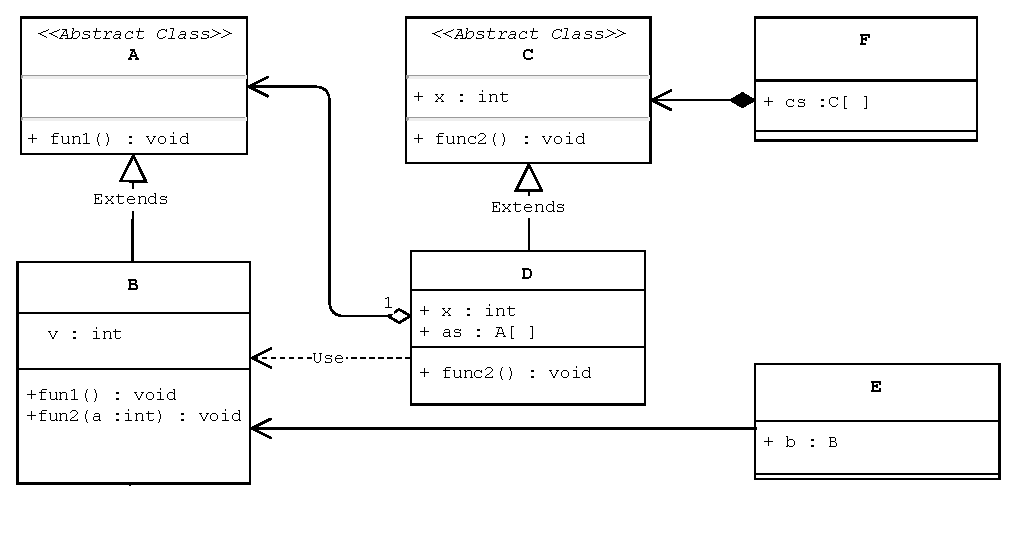
\includegraphics[width=0.47\textwidth]{class_diagram.eps}
	}
	\hspace{0em}	
	\subfigure[Phenotype]
	{
		\label{fig:dtlz710nsgaiiifigure3d}
		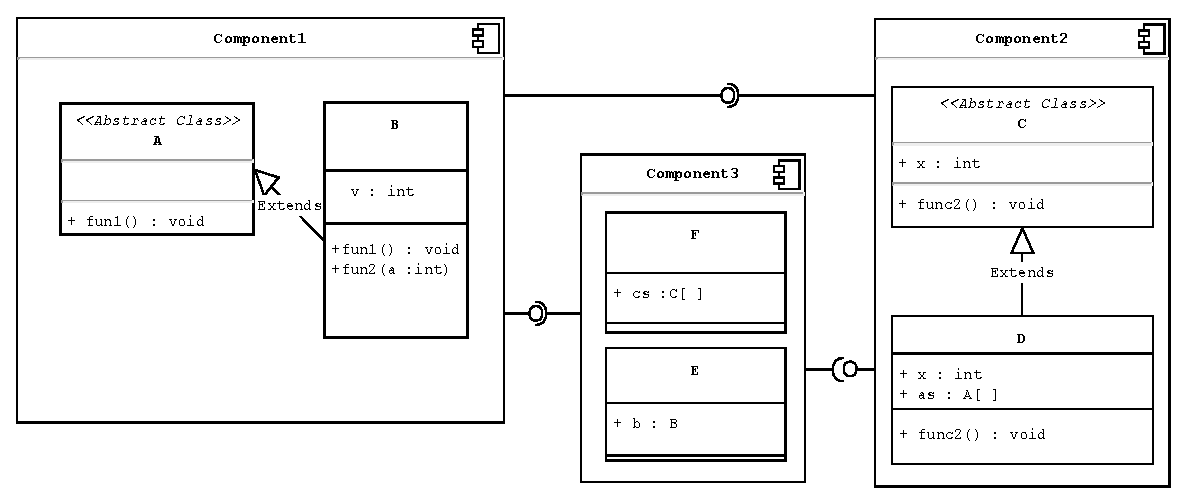
\includegraphics[width=0.47\textwidth]{phenotype.eps}
	}	
%	\hspace{0em}
%	\subfigure[MOEA/D]
%	{
%		\label{fig:dtlz710moeadfigure}
%		\includegraphics[width=0.170\textwidth]{figures/experiments/dtlz/moeaddtlz7_10.eps}
%	}	
%	\hspace{0em}	
%	\subfigure[FD-NSGAII]
%	{
%		\label{fig:dtlz710zhenanfigure}
%		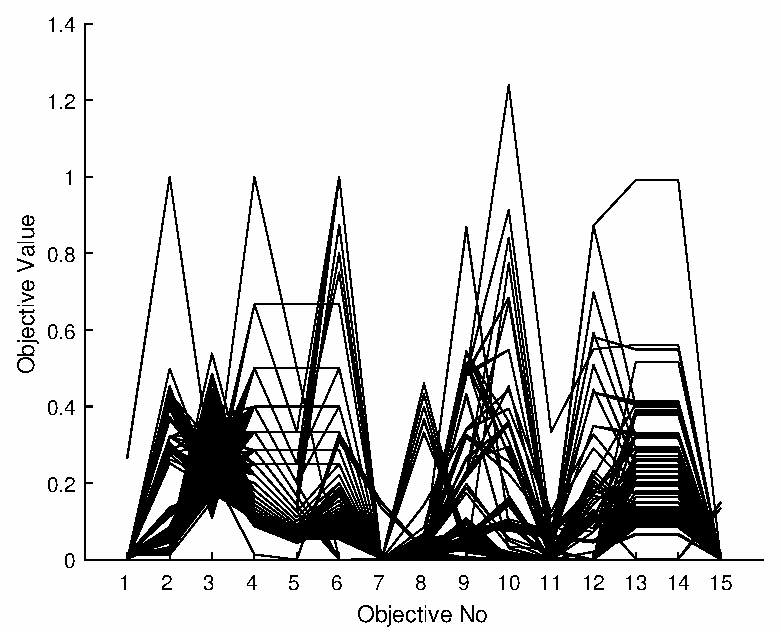
\includegraphics[width=0.170\textwidth]{pp/ical4j_ENSGAIII_15_1.eps}
%	}	
%	\hspace{0em}
%	\subfigure[HypE]
%	{
%		\label{fig:dtlz710hypefigure}
%		\includegraphics[width=0.170\textwidth]{figures/experiments/dtlz/hypedtlz7_10.eps}
%	}	
%	\hspace{0em}	
%	\subfigure[SDE]
%	{
%		\label{fig:dtlz710sdefigure}
%		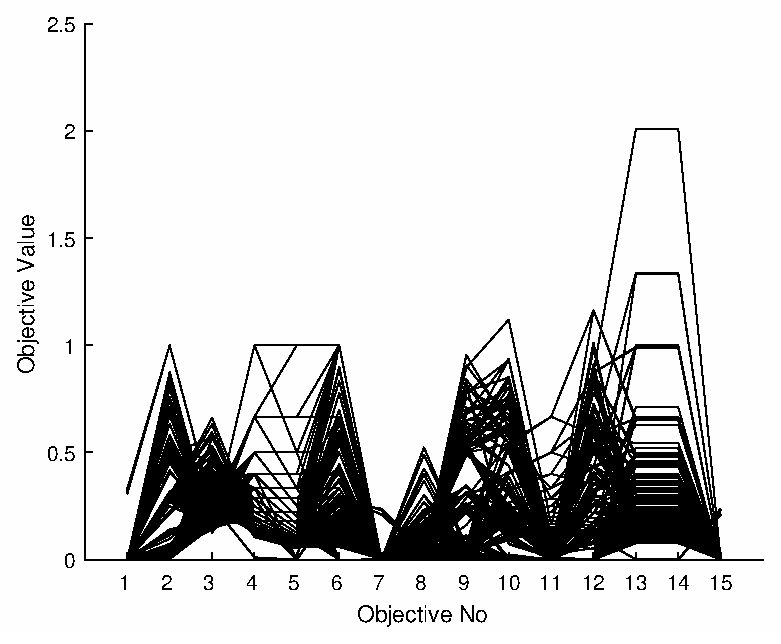
\includegraphics[width=0.170\textwidth]{pp/ical4j_NSGAIII_15_20.eps}
%	}	
%	\hspace{0em}
%	\subfigure[PICEAg]
%	{
%		\label{fig:dtlz710piceagfigure}
%		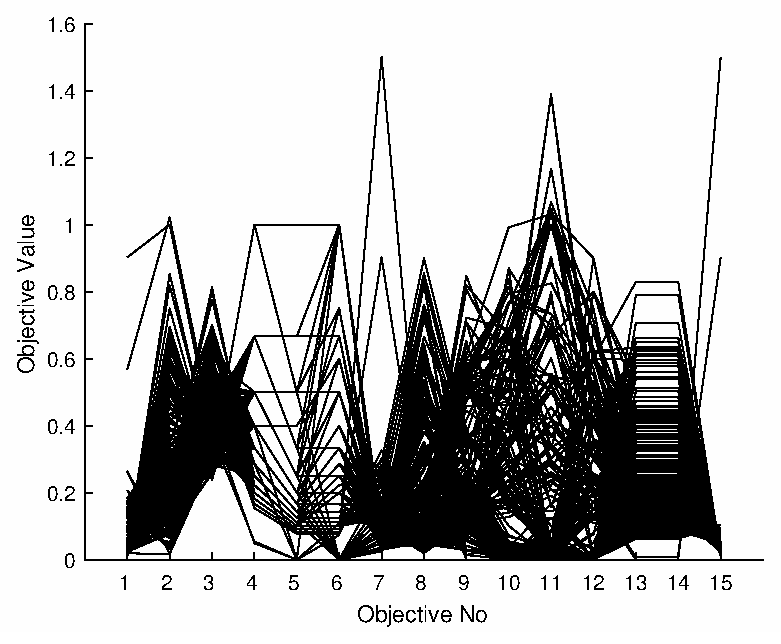
\includegraphics[width=0.170\textwidth]{pp/xapool_NSGAIII_15_20.eps}
%	}	
\caption{An Example of an Architecture}
\end{figure*}


%\begin{figure*}[!h] \label{phenotype}
 % 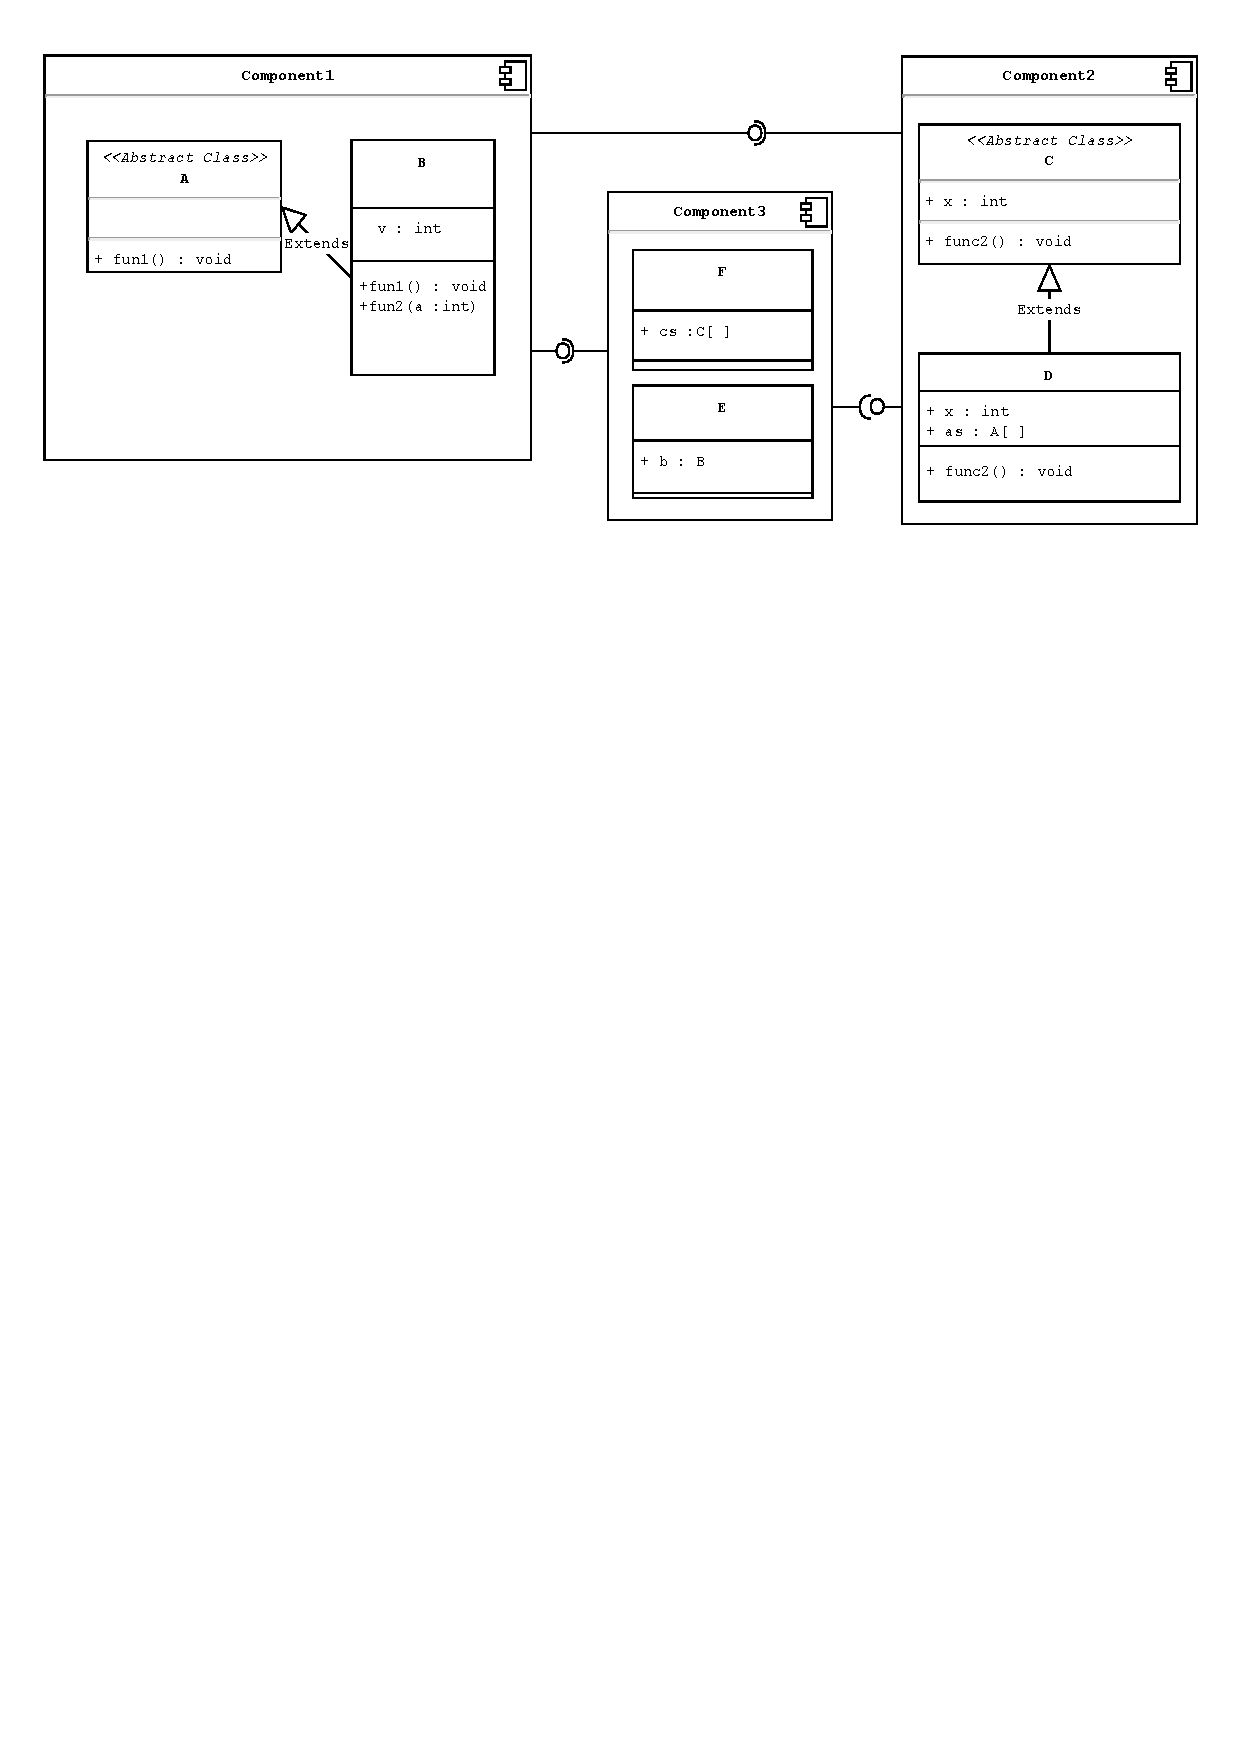
\includegraphics[width=\linewidth]{phenotype.png}
%  \caption{Genotype}
%  \label{fig:genotype}
%\end{figure*}


In our search problem, the initial state is a Genotype. The actions are to generate new genotype by moving a UML class from one component to another, and the goal is to get a genotype that will provide better performance, maintainability, and security of the software.

\textbf{Problem formulation}:
\begin{itemize}
\item \textbf{Initial State} : Create a solution set by randomly generated Genotypes from UML classes and their relations.

\item\textbf{Actions}: Perform some crossover and mutation over  
solution set and generate new child genotypes.
\item \textbf{Transition Model}: From old parent and new child genotypes, keep the best ones using some metrics value.
\item \textbf{Goal}: Generate the optimal solution set

\end{itemize}


To measure the performance, maintenance and security of the software, we proposed some metrics. Our proposed metrics are mainly two categories: some are related to performance and maintenance and others are linked to the security of the software.


\subsection{Metrics Related to Performance and Maintenance}
We have considered  10 metrics which are related to performance and maintenance of a software. Primarily the main objective of a software is to serve its functional requirements. Software architecture is designed in this manner so that it serves those requirements. Besides those requirements, some non-functional requirements such as performance, maintenance is also considered. Hence, while designing a software architecture, architects have to deal with some aspects of that software like understanding, reuse, construction, evaluation, analysis, and management\cite{garlan2000software}. Here, we considered some metrics those are not directly tied to the functional requirements, but important for other non-functional requirements. Some metrics are important for modularity. Those ensure smooth and fluent development process with future modification, inclusion, and correction. 
In software engineering, there are some core parts those can be used for other software development. Hence, some metrics are selected to obtain reusability.
We have explored other research papers for metrics. There are some similar types of metrics and some metrics have no context in our problem. Considering those criteria, we selected 10 metrics.
 \newline
For each metric calculation,  we assume the number of components of the architecture is $n$. 

\begin{enumerate}
\item \textbf{Intra-modular Coupling Density (icd):} This metric represents the ratio of a internal and external interactions of a component. This metric was proposed by Gupta~\cite{gupta2012optimization}. Let us assume that $\#classes_{total}$ be number of total classes of genotype and $\#classes_{i}$ be the number of component $i$. Also let $c^{in}_i$ and $c^{out}_i$ denote the number of inner and outer connections of component $i$ respectively and  Intra-modular Coupling Density of component $i$ is $icd_{i}$. Then,
\begin{equation}\label{icd_eq_i}
icd_{i}=\frac{\#classes_{total}-\#classes_{i}}{\#classes_{total}}\times\frac{c^{in}_i}{c^{in}_i+c^{out}_i} 
\end{equation}\\
For all components,
\begin{equation}\label{icd_eq}
icd=\frac{1}{n}\sum{icd_{i}}
\end{equation}
For other metrics we shall follow same convertion.

\item \textbf{External Relations Penalty (erp):} This metric is proposed by Krogmann\cite{krogmann2012reconstruction}. This is the weighted sum of different types of relations. For two component pair $i$ and $j$, let us assume that, $(w_{as},n_{as_{ij}})$ be the weight and the number of relation for Associations. Similarly let $(w_{ag},n_{ag_{ij}})$, $(w_{co}, n_{co_{ij}})$, $(w_{co} ,n_{co_{ij}})$, $(w_{ge},n_{ge_{ij}})$ be  the weight and the number of relation for Aggregation, Composition, and Generalization respectively. Then $erp$ is computed as:
\begin{equation}\label{erp_eq}
 erp=\sum_{i=1}^{n}{\sum_{j=i+1}^{n}}{w_{as}n_{as_{ij}}+w_{ag}n_{ag_{ij}}+w_{co}n_{co_{ij}}+w_{ge}n_{ge_{ij}}}
\end{equation}

\item \textbf{Cohesion inside a Component (coc):}
This metric represents the ratio of internal connection and the number of classes of a component to find the cohesion inside a component.Total $coc$ will be average $coc$ of all components. Let us assume that, for component $i$ the number of classes be $\#class_{i}$ and  the number of internal connections be $\#connection^{in}_{i}$ and cohesion of that component be $coc_{i}$. Then,
\begin{equation}\label{coc_eq}
 \begin{array}{l}
coc_{i}=\frac{\#connection^{in}_{i}}{\#classes_{total}} \\
coc=\frac{1}{n}\sum{coc_{i}}
\end{array}
\end{equation}

\item \textbf{Link Criticality (lc):} Link Criticality is defined as a condition in which a component has many links to other components. There is a $threshold_{link}$ limit for the number of links for a component. This metric is proposed by Narasimhan and Hendradjaya  \cite{narasimhan2007some}. Let us assume that $\#component_{link\_crtiticality}$ and $\#component_{total}$ be  the number of components which have crossed $threshold$ and total number of component respectively. Then, Link Criticality:
\begin{equation}\label{lc_eq}
lc=\frac{\#component_{link\_criticality}}{\#component_{total}\textbf{}}
\end{equation}

\item \textbf{Size Criticality (sc):} Size Criticality is defined as a condition in which a component has many classes. There is a $threshold_{size}$ limit for the number of classes. This metric is proposed by Narasimhan and Hendradjaya  \cite{narasimhan2007some}. Let us assume that, $\#component_{size\_crtiticality}$ and $\#component_{total}$ be the  number of components which have crossed size limit $threshold$ and total number of components respectively. Then, size Criticality:
\begin{equation}\label{sc_eq}
sc=\frac{\#component_{size\_criticality}}{\#component_{total}}
\end{equation}

\item \textbf{Interaction Density (id):} A component provides and receives some connections. Interaction Density (id) is the ratio of connection provided and total connection. This metric is defined by Matrin~\cite{martin1994oo}. Later it was proposed by Sant'Anna \textit{et. al.}~\cite{sant2007modularity}. Let us assume that, for component $i$,
$\#con_{provide}$ be the number of provided connections and $\#con_{receive}$ be the number of received connections. Then,
\begin{equation}\label{id_eq}
 \begin{array}{l}
id_{i}=\frac{\#con_{provide}}{\#con_{provide}+\#con_{receive}} \\\\
id=\frac{1}{n}\sum{id_{i}}
\end{array}
\end{equation}


\item \textbf{Encapsulation (enc):} This metric measures the ratio of hidden classes with respect to component. This metrics is proposed by Bansiya and Davis\cite{bansiya2002hierarchical}. For component $i$ let the number of inner classes and total classes be $\#classes_{inner}$ and $\#classes_{total}$ respectively. Encapsulation is calculated for that component by the ratio of these values. Overall encapsulation is calculated by averaging encapsulation of all components. Hence, encapsulation for Component $i$:

 \begin{displaymath}
enc_{i}=\frac{\#classes_{inner}}{\#classes_{total}} 
 \end{displaymath}
Overall encapsulation:

\begin{equation} \label{enc_eq}
enc=\frac{1}{n}\sum{enc_{i}}
\end{equation}



\item \textbf{ McCabe's Cyclomatic Complexity (cc):} Cyclomatic complexity is  used to indicate the complexity of a architecture. This metric is proposed by McCabe and Thomas~\cite{mccabe1976complexity}. Let us assume that  $\#con$ be the number of connections of  an architecture, $\#com$ be the number of components, and  $\#Con\_com$ be the connected components. Then Cyclomatic complexity will be:
\begin{equation}\label{cc_eq}
cc=\#con - \#com + \#con\_com 
\end{equation}

\item \textbf{Groups/Components Ratio (gcr):}
The metric is the ratio of number of connected classes ($\#classes_{connected}$) and number of components ($\#component$). Then,
\begin{equation}
gcr=\frac{\#classes_{connected}}{\#component}
\end{equation}
It is proposed by  Narasimhan and Hendradjaya\cite{narasimhan2007some}.

\item \textbf{Abstractness (abs): }For a component, abstractness is the ratio between the number of abstract classes and total classes. Abstractness of full architecture is measured by averaging abstractness of all components. This metric is proposed by Krogmann\cite{krogmann2012reconstruction}. Let us assume that, for component $i$ $\#classes_{abstract}$ be the number of abstract classes, and $\#classes_{total}$ be the number of total classes. Then,
\begin{equation}\label{abs_eq}
 \begin{array}{l}
abs_{i}=\frac{\#classes_{abstract}}{\#classes_{total}} \\
abs=\frac{1}{n}\sum{abs_{i}}
\end{array}
\end{equation}








\end{enumerate}



\subsection{Metrics Releted to Security}
Security is recently considered very important part of  software engineering. In genotype representation, each component works individually and  communicate with each other through the connection between them. 
%Here outer a malicious component can set up to make connecting one of the components of a software and raise a security worry.  
Careful connection set up between different components can bring down this security concern. Hence, we proposed five security metrics to determine the risk of a genotype. \\ 
First, we have to identify \textbf{Critical Classes}. A class will be called critical if any of its classified private attributes can be modified from outer side of that class \cite{alshammari2010security}. A component with the critical class will be considered as a critical component. Those components have higher security  vulnerabilities . The formation and connection of that component must be set carefully to reduce those  vulnerabilities .

For all metrics bellow, let us assume that, the total number of component be $n$ and $i$ represents $i^{th}$ component.

\begin{enumerate}
\item \textbf{Composite-Part Critical Classes (CPCC):} If any class has one or many classified attributes which are the object of a critical class, then that class will have critical security concern. Here critical class provides either composition, or aggregation, or association related to that class. If both this class and critical class belong to the same component, then risk of attack from another component will be minimized. \\
Let us assume that, for component $i$, $cc_{i}$ be the set of critical classes and $CPRCC_{inside}(x)$ be a function where $x$ is critical class. This function returns number of classes those are in the same component of x and they receive composite part relation from critical class $x$. 
$CPRCC_{total}(x)$ is returns total number of classes  which receive composite similar relation from critical class $x$.

\begin{equation}\label{cpcc_eq}
\begin{array}{l}
cpcc_{i}=\sum_{cc \in cc_{i}}{\frac{CPRCC_{inside}(cc)}{CPRCC_{total}(cc)}}\\\\
cpcc=\frac{1}{n}\sum_{i=1}^{n}{cpcc_{i}}
\end{array}
\end{equation}

\item \textbf{Critical Classes Extensibility (CCE):} If any class extends or inherits a critical class,  that class also  has security concerns because that class can be accessed through the critical class. This type of classes receive the generalization relationship from a critical class. Therefore, like CPCC CCE is a metric to keep critical class and it extends class in a same component. 
$GRCC_{inside}(x)$ is a function where $x$ is critical class. This function returns number of classes those are in the same component of x and they receive generalization relation from critical class $x$.

$GRCC_{total}(x)$ is similar., but it returns total number of classes those receive generalization relation from critical class $x$.
\begin{equation}\label{cce_eq}
\begin{array}{l}
cce_{i}=\sum_{cc \in cc_{i}}{\frac{GRCC_{inside}(cc)}{GRCC_{total}(cc)}}\\\\
cce=\frac{1}{n}\sum_{i=1}^{n}{cce_{i}}
\end{array}
\end{equation}

\item \textbf{Critical Classes Coupling (CCC):} Previously we have defined that critical class is a class which  contains classified private attributes that can be modified by other classes. Now let  $AC_{i}$ and $CC_{i}$ be respectively  set of all classes and critical classes define in a component $c_{i}$. \\
$cc$ is a critical class of $c_{i}$.
So $cc \in CC_{i}$ \\
$CA_{cc}$ is the set of critical classified attributes of a critical class $cc$. $\alpha(CA_{cc})$ is the set of classes those modify critical private attributes of $cc$. In this case, the genotype will be more secure if  more number of classes of $\alpha(CA_{cc})$ belong to the same component of $cc$.
\begin{equation}\label{ccc_eq}
 \begin{array}{l}
ccc_{i}=\sum_{cc \in CC_{i}}{\frac{n(\alpha(CA_{cc}) \cap CA_{i})}{n(\alpha(CA_{cc})}}\\\\
ccc=\frac{1}{n}\sum{ccc_{i}}
\end{array}
\end{equation}

\item \textbf{Classified Methods Extensibility (cme):} 
Malicious components can also modify critical information of any class by extending non-finalized classified methods. This metric is the ratio of extendable non-finalized methods inside a component and total extendable non-finalized methods. This ratio is the $cme$ value for a component. Overall $cme$ is mean of all components.\\
Lets assume that for component $i$, $\#enfm_{inside}$ and $\#enfm_{total}$ are  extendable non-finalized methods inside a component and total extendable non-finalized methods respectively.
\begin{equation}\label{cme_eq}
 \begin{array}{l}
cme_{i}=\frac{\#enfm_{inside}}{\#enfm_{total}} \\
cme=\frac{1}{n}\sum{cme_i}
\end{array}
\end{equation}


\item \textbf{Classified Attribute Extensibility (cae):}
Similar to $cme$, $cae$ is the ratio of extendable non-finalized attributes inside a component and total extendable non-finalized attributes.\\
Lets assume that for component $i$, $\#enfa_{inside}$ and $\#enfa_{total}$ are  extendable non-finalized attributes inside a component and total extendable non-finalized attributes respectively.
\begin{equation}\label{cae_eq}
 \begin{array}{l}
cae_{i}=\frac{\#enfa_{inside}}{\#enfa_{total}} \\\\
cae=\frac{1}{n}\sum{cae_i}
\end{array}
\end{equation}


  
\end{enumerate}
 


\section{Methodologies}
\label{sec:methodologies}

\subsection{Overall Process}
We have formulated the discovery of the software architecture as a search-based optimization problem. Our goal is to find optimized architecture (class diagram) in terms of $15$ conflicting performance metrics. The problem is thus formulated as a Many Objective Optimization Problem (MaOP) and solved using evolutionary Many-Objective Optimization algorithms. The interesting property of these optimizers is that they can offer comparability among solutions beyond Pareto dominance and can be adapted to solve various classes of problems. One such modern state of the art many objective optimizer is NSGA-III, which has been widely accepted in the research community. NSGAIII utilizes reference point based clustering and niche count based selection procedure to balance diversity and convergence among solutions. While the basic NSGAIII works well for standard MaOPs, they do not however incorporate any problem specific domain knowledge to the algorithm. With that motivation, we have replaced the niching based selection procedure of NSGAIII with a Fuzzy logic based selection scheme where problem specific knowledge have been incorporated. The proposed algorithm $F$-NSGAIII has been found to be better performing than the original one for this particular problem and an in depth analysis at experimental studies section conforms with our theoretical reasonings.

%Recently, the MaOP has gained popularity among researcher due to their frequent appearance in real world problem. 


\subsection{Adaptation of NAGAIII}
\label{subsec:pseudocode}

The basic algorithm of NSGAIII starts with a randomly generated parent population $P_t$ of $N$ solutions and a set of generated/supplied reference points $R^p$. It then creates an offspring population $Q_t$ of size $N$ by applying crossover and mutation. The solutions are combined $C_t = P_t \bigcup Q_t$ (of size 2N) and ranked into different Pareto fronts ($F_1, F_2, \cdots, F_n$). Solutions within a particular Pareto front are non-dominated to each other and a lower ranked Pareto front represents that solutions in that front are less dominated than higher ranked ones. For elite preservation thus each non-dominated Pareto fronts is selected to construct a new population $S_t$, starting from $F_1$, until the size of $S_t$ is equal to $N$ or for the first time exceeds $N$. Let us say the last level included is the $l$-th level. Thus, all solutions from level $(l + 1)$ onwards are rejected from the combined population $C_t$. 

If the population size in $S_t$ are Based on the euclidean distance between a solution and the reference points population
It then adaptively constructs $m$ fuzzy membership functions i.e., one function for each objective 
and utilizes them to compute dominance degrees of the solutions. Finally, $F$-NSGAIII assigns fitness to the solutions and selects the best ones from different clusters in a round-robin fashion to from a new population $P_{t+1}$ for the next generation.  
We summarize the steps of our method in Algorithm 1, which are explained further in the following subsections.


 %%%%%%%%%%%%%%%%Complete Algorithm%%%%%%%%%%%%%%%%%%%%%%%%

 \begin{algorithm}[!h]
	
 	\textbf{Input:} $R^p$ (generated reference points or supplied points), $P_t$ (parent population of $t$-th generation), $N$ (population size)\\
 	\textbf{Output:} $P_{t+1}$
	
 	\begin{algorithmic}[1]
		\State $Q_t \gets $ Recombination and Mutation on $P_t$
 		\State $C_t \gets P_t \cup Q_t$				 	
 		\State $(F_1,F_2,....)$=Non-Dominated-Sort$(C_t)$
        
        \State $S_t \gets \phi , i\gets 0$
        \While {$|S_t| \le N$}
        \State $S_t \gets S_t \cup F_i$
        \State $i \gets i+1$
        \EndWhile
        \State Last-Front to be included: $F_l \gets F_i$
        \If {$|S_t| = N$}
        \State $P_{t+1} \gets S_t$
        \Else
        \State $P_{t+1} \gets \cup _{i=1}^{l-1}F_i$
        \State $\pi({\textbf{s})}$=\textbf{Associate}$(F_l,R^p)$ \% $\pi({\textbf{s}})$:closest reference point 
        \State \textbf{Selection}($F_l,R^p,\pi,P_{t+1}$,N)  \% Select Remaining points from last front
        
        \EndIf
        
        
		
	\end{algorithmic} 
	
	\caption{Generation $t$ of $F$-NSGAIII}
	
 	\label{alg:completeAlgorithm}
 \end{algorithm}

\subsection{Crossover and Mutation}
Crossover and mutation operators generate new possible genotypes from an existing genotypes. Here we have used five mutation operation. Firstly parents are selected randomly from the current population. Then from that parents, offsprings are generated using five mutations. Those mutations are:
\begin{enumerate}
\item Adding a new component to the architecture. Next some random classes are chosen from existing components and those classes are added to the new component. Finally, connections are set with new component and there might be necessity to correct some other connections.
\item Removing a component from architecture. UML classes of the component ,which is removed, are then distributed randomly to other existing components. Then other components' connection with that component are reset according to new architecture.
\item Merging two components of an architecture. Here connections of those components are attached to the new merged component if they have come from another component. Connections between two merging components will be considered as internal connections of the new component.
\item Spliting a component into two components. Here, UML classes of older component are distributed to new two components randomly. Then outer connections of divided components are attached to newly built component according to their UML classes. Some internal connections of old divided class will be set as external connections of new components.
\item Moving a class from one component to another component.  After this operation, some connections due to that class are moved from the source component to the destination component. Internal connections of the class, which has moved, will be set as external connection to destination component. External connections of the destination component due to this class will be set as internal connections.

\end{enumerate}
Figure \ref{mutation} is an example of a mutation. This mutation is performed by moving a class from Figure \ref{geno_example}. 
\begin{figure*} [!h] \label{mutation}
  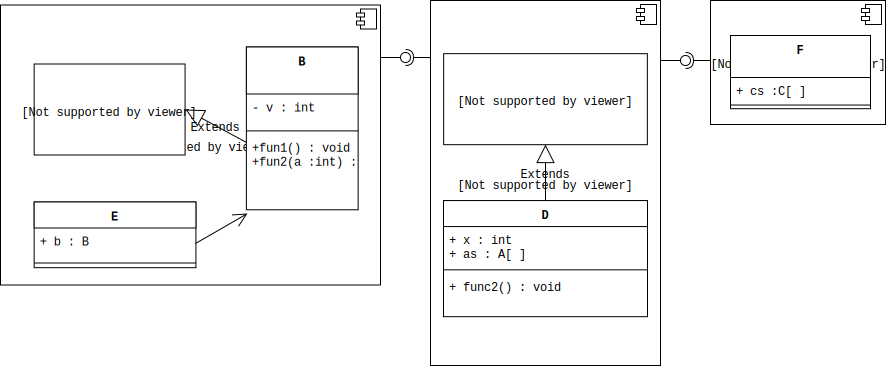
\includegraphics[width=\linewidth]{phenotype_cross.eps}
  \caption{Genotype after Mutation}
\end{figure*} 


%\begin{figure*} [!h]
 % \includegraphics[width=\linewidth]{cg1.png}
 % \caption{Genotype after Mutation}
%\end{figure*}


Now any mutation of those five will be selected with weighted probability and that mutation will be executed to generate offspring. Because of the context of the problem there is no suitable crossover operation for this problem. That is why there will not be any crossover execution.

\subsection{Clustering}
For clustering, we have used the same procedure of NSGAIII. After normalizing each objective value, we need to associate every member of the population to a reference point. A reference line corresponding each reference point is defined in the hyper plane by connecting the origin and reference point. Then we calculate the perpendicular distance of each solution member, of $C_t$ from each reference line. For each population member a reference point is assigned whose reference line has the shortest distance to that population member. 

\begin{algorithm}[!h]
	
 	\textbf{Input:} $C_t,R^p$\\
 	\textbf{Output:} $\pi(\textbf{s} \in C_t)$
	
 	\begin{algorithmic}[1]
		\For {each reference point $\textbf{r} \in R^p$}
        	\State Compute reference line $\textbf{w}=\textbf{r}$
 		\EndFor
        \For {each $\textbf{s} \in C_t$}
        	\For {each $\textbf{r} \in R^p$}
            	\State Compute $d^\perp=\parallel(\textbf{s}-\textbf{w}^\perp \textbf{sw}/\parallel \textbf{w} \parallel ^2)\parallel$
            \EndFor
            \State $\pi(\textbf{s})=\textbf{w}:argmin_{\textbf{w} \in R^p}d^\perp(\textbf{s},\textbf{w})$
      
  
        
        \EndFor
		
	\end{algorithmic} 
	
	\caption{Associate($C_t$,$R^p$) procedure}
	
 	\label{alg:associate}
 \end{algorithm}




\subsection{Ranking}
For ranking, we have modified NSGAIII algorithms. First, we rank each solution using Non-Dominated Ranking like NSGAIII. By this ranking, we get different level of Front. However, we ranked solutions in  the last-front in a different way than NAGAIII . To rank solutions in  the last-front we have defined a comparator procedure which will compare two solutions and return the best of them. Now, as each solution is a set of 15 contradictory objectives, there is a very high probability that they will be non-dominated. NSGAIII counts the number of solutions assigned to each reference point. They call it Niche count. They select solution with this Niche count. When Niche count becomes zero, NSGAIII selects a random solution. We hope that we can get improved result by selecting solutions using objective-wise comparison rather selecting them randomly. To compare two solutions objective-wise, we have calculated their Gaussian distance. In our problem the difference between each normalized objective of two solution varies from [-1,1].
For minimizing problem difference -1 indicates that  the first solution is much better on that objective and 1 indicates that the first solution is worse. 
To find the Gaussian distance between those two solutions on an objective, we used following half Gaussian function( Figure ref{fig:gaussian}).

\begin{equation}
G(x)=\frac{1}{\sqrt{2\pi\sigma^2}} e^{-\frac{(x-\mu)^2}{2\sigma^2}}
\end{equation}
here $x$  the is difference between same normalized objective of two solutions and
\begin{equation}
\sigma=0.388
\end{equation}
\begin{equation}
\mu=-1
\end{equation}

\begin{figure} [!h] \label{fig:gaussian}
  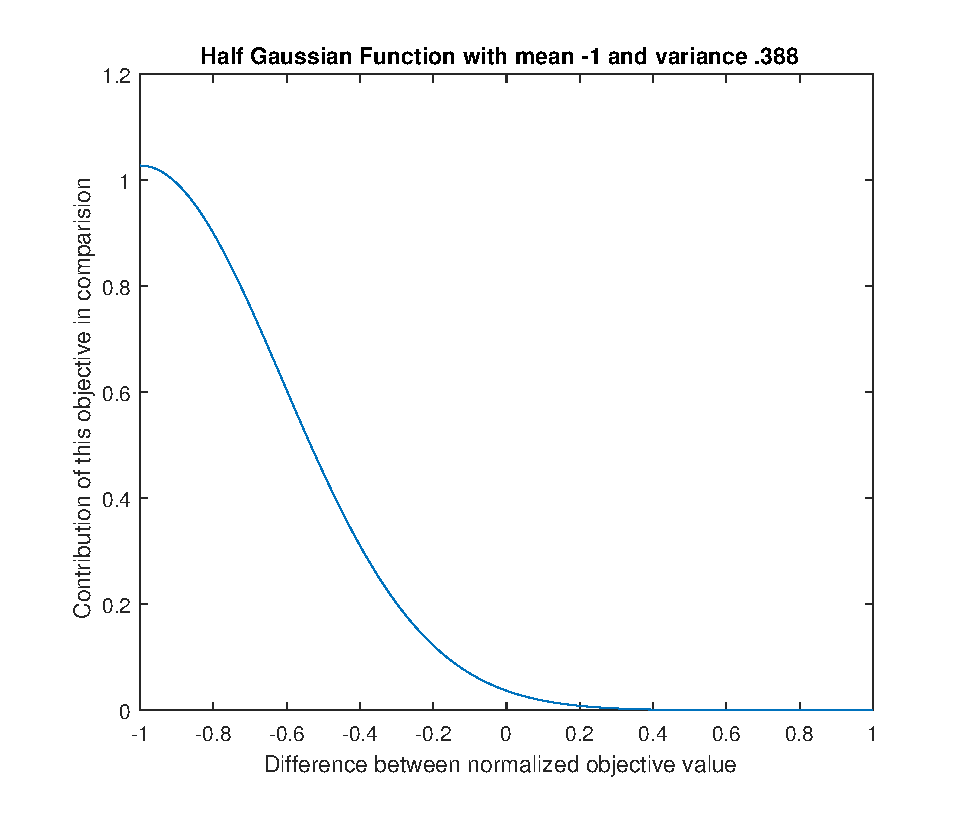
\includegraphics[width=\linewidth]{gaussian.eps}
  
  \caption{Half Gaussian Function}
\end{figure}
Now between two solutions, let $\mathbf{s}_1$ and $\mathbf{s}_2$ are respectively normalized objective of them and $ \tilde{f_i}(\mathbf{s})$
returns $i^{th}$ normalized objective of a solution.  We  may now derive $d_1$ and $d_2$ where $d_1$ is the Gaussian distance of solution $\mathbf{s}_1$ from solution $\mathbf{s}_2$ and similarly, $d_2$ is the Gaussian distance of solution $\mathbf{s}_2$ from solution $\mathbf{s}_1$.
\begin{equation}
    d_1=\prod_{i=1}^{m}G( \tilde{f_i}(\mathbf{s}_1)-\tilde{f_i}(\mathbf{s}_2)) 
\end{equation}
\begin{equation}
    d_2=\prod_{i=1}^{m}G( \tilde{f_i}(\mathbf{s}_2)-\tilde{f_i}(\mathbf{s}_1))
\end{equation}
Now if $d_1 > d_2$, we can say that $\mathbf{s}_1$ is better that $\mathbf{s}_2$ and vice versa.

We also measure solution distance from its clustered reference point. To find this distance, first we normalize reference point. Then in hyper-space, we take the dot product of solution and their perpendicular distance. 
Dot product of normalized solution and reference point is $d^d$ and $d^{\perp}$ is the perpendicular distance between them. Both $d^d$ and $d^{\perp}$ are ranged  in [0,1]. However, Gaussian distance, $d^g$ is valued too small. Hence, we take the  $log$ summation of them. Then, we normalized them to get Gaussian distance($d^g$)
\begin{displaymath}
\log d_1=\sum_{i=1}^{m} \log G( \tilde{f_i}(\mathbf{s}_1)-\tilde{f_i}(\mathbf{s}_2))
\end{displaymath}
\begin{displaymath}
\log d_1=\sum_{i=1}^{m} \log G( \tilde{f_i}(\mathbf{s}_1)-\tilde{f_i}(\mathbf{s}_2))
\end{displaymath}
\begin{equation}
d_{1}^g=\frac{\log d_1}{\log d_1 + \log d_2} 
\end{equation}
\begin{equation}
d_{2}^g=\frac{\log d_2}{\log d_1 + \log d_2} 
\end{equation}


Finally, comparing weighted sum of those values, we decide which solution is better. We present this approach in Algorithm \ref{alg:Comparetor}






\begin{algorithm}[!ht]
	
 	\textbf{Input:} $\textbf{s}_1 \in C_t,\textbf{s}
_2 \in C_t,\pi(\textbf{s} \in C_t)$\\
 	\textbf{Output:} $f$
	
 	\begin{algorithmic}[1]
    \State set $w^g,w^d,w^{\perp}$ according to problem specification
    \State $\sigma \gets 0.388$
    \State $\mu \gets -1$
    \State $d_1 \gets 0$
    \State $d_2 \gets 0$
    \For {$i \gets 1 {\ }TO {\ } m$ }
    \State $x \gets \tilde{f_i}(\mathbf{s}_1)-\tilde{f_i}(\mathbf{s}_2) $
    \State $d_1 \gets d_1+\log(G(x))$
     \State $d_2 \gets d_2+\log(G(-x))$
    
    \EndFor
    \State $d_{1}^g \gets \frac{d_1} {d_1+d_2}$
    \State $d_{2}^g \gets \frac{d_{2}^g} {d_1+d_2}$
    \State $\mathbf{w} \gets \pi(\mathbf{s}_1)$
    \State $\mathbf{\tilde{w}} \gets \mathbf{w} / \parallel \mathbf{w} \parallel$
    \State $d_{1}^d \gets \mathbf{\tilde{w}} \cdot \mathbf{s}_1$
    \State $d_{1}^d \gets \mathbf{\tilde{w}} \cdot \mathbf{s}_2$
    \State $d^{\perp}_1 \gets \parallel(\mathbf{s}_1-d_1^d \mathbf{\tilde{w}}) \parallel $
        \State $d^{\perp}_2 \gets \parallel(\mathbf{s}_2-d_2^d \mathbf{\tilde{w}}) \parallel $
        
        \State $d_1 \gets w^g\times d^{g}_1+ w^d \times d^{d}_1 + w^{\perp} \times d^{\perp}_1 $
        \State $d_2 \gets w^g\times d^{g}_2+ w^d \times d^{d}_2 + w^{\perp} \times d^{\perp}_2 $
         \State $f \gets 0$
    \If {$d1 > d2$}
    \State $f \gets -1$
    \EndIf
    \If {$d1 < d2$}
     \State $f \gets 1$
    \EndIf
   
    
    
		
	\end{algorithmic} 
	
	\caption{Comparator($\textbf{s}_1,\textbf{s}_2,\pi$) procedure}
	
 	\label{alg:Comparetor}
 \end{algorithm}





\subsection{Selection}
After Non-dominated ranking, we select solutions of all front expect last Pareto-Front. For solutions in the last Pareto-Front we select the best solution using Comparator function defined in Algorithm \ref{alg:Comparetor}. 
Then we make a set of solutions for each reference points and add the best solution to $P_{t+1} $.
  

\begin{algorithm}[!ht]
	
 	\textbf{Input:} $C_t,R^p,\pi(\mathbf{s} \in C_t),P_{t+1},N$\\
 	\textbf{Output:} $P_{t+1}$
	
 	\begin{algorithmic}[1]
    \State $added \gets 0$
    \For {each $\mathbf{s} \in C_t$}
    \State $\mathbf{w} \gets \pi(\mathbf{s})$
    \State get reference point $\textbf{r}$ from reference line $\mathbf{w}$
    \State $L \gets $ set of solutions assigned to reference point $\textbf{r}$
    \State $\mathbf{s}_b \gets \mathbf{s}$
    \For {each $\mathbf{s}_c \in L$}
    \State $ f \gets Comparator(\mathbf{s}_c,\mathbf{s}_b,\pi)$
    \If {$f =-1$}
    \State $\mathbf{s}_b \gets \mathbf{s}_c$
    \EndIf
    
    \EndFor
    \State $P_{t+1} \gets P_{t+1} \cup \mathbf{s}_c$
    \If {$|P_{t+1}|=N$}
    \State $return$
    \EndIf
    \State $C_{t} \gets C_{t}\backslash best $
    
    
    
    \EndFor
	\end{algorithmic}
    \caption{Selection($C_t,R^p,\pi,P_{t+1}$) procedure}
 	\label{alg:selection}
 \end{algorithm}
 


\section{Experiments}
\subsection{Dataset Formulation}
In our research, we try to develop an automated method to discover the best fitted underlying architecture to serve its functional requirements as well as nonfunctional requirements. This work will help software architects to find a good architecture and find its best equivalent alternative for the changes during the development process. The input of our work is a UML class diagram of a software. To get UML class diagram, we have used Open Source Java project from github and other sites. Then we have reversed engineered those codes to UML class diagram. 

\subsection{Algorithm Implementation}
In this part, we have solved a Search Based Software Engineering (SBSE) problem using Evolutionary Many Objective Algorithms.
As parameter of those Evolutionary Many Objective Algorithms, we have considered:
\begin{displaymath}\label{population_size}
Population\_Size=320
\end{displaymath}
\begin{displaymath}\label{ref_point}
Reference\_Point\_Size=640
\end{displaymath}
\begin{displaymath} \label{max_gen}
Max\_Generation=100
\end{displaymath}
\begin{displaymath} \label{run_num}
Run\_Number=5
\end{displaymath}



At the very beginning, we generate 320 random genotypes from a class diagram and they are added to the solution set. Then we have calculated 15 evaluation metrics for each genotype. Here some metrics are minimizing objectives, and some are maximizing objectives. Which metrics are minimizing objectives, and which are maximizing objectives vary according to the requirement of the software. Again, all security metrics must be set as minimizing. Following a Table~\ref{tb:metrics table} shows whether a matrices is only maximizing or only minimizing or both. 
Here, $\updownarrow$ means metrics are can  be either maximizing or minimizing. This will be decided according to the requirement of the software. Only $\uparrow$ or $\downarrow$ means, those metrics are only maximizing or minimizing respectively.  
\begin{table}[!h]
\caption{Metrics Table}

\begin{center}

\begin{tabular}{ |c|c|c| } 

% % \hline
% $icd$ &  $\updownarrow$  & $\uparrow$ &
% $erp$ & $\updownarrow$ &  $\downarrow$\\ \hline
% $coc$ & $\updownarrow$ &  $\uparrow$ &
% $lc$ & $\updownarrow$ &  $\downarrow$\\ \hline
% $sc$ & $\updownarrow$ &  $\downarrow$ &
% $id$ & $\updownarrow$ &  $\downarrow$\\ \hline
% $enc$ & $\updownarrow$ &  $\downarrow$ &
% $cc$ & \textbf{$\downarrow$} &  $\downarrow$\\ \hline
% $gcr$ & $\updownarrow$ &  $\downarrow$ &
% $abs$ & $\updownarrow$ &  $\downarrow$\\ \hline
% $cpcc$ & \textbf{$\downarrow$} & $\downarrow$ &
% $cce$ & \textbf{$\downarrow$} & $\downarrow$ \\ \hline
% $ccc$ & \textbf{$\downarrow$} & $\downarrow$ &
% $cme$ & \textbf{$\downarrow$} & $\downarrow$ \\ \hline
% $cae$ & \textbf{$\downarrow$} & $\downarrow$ \\ \hline


 \hline
 Metrics Name & In General & In Our Experiment\\ \hline
$icd$,$id$, $gcr$,$abs$ &  $\updownarrow$  & $\uparrow$ \\ \hline
$coc$ & $\uparrow$ &  $\uparrow$ \\ \hline
$erp$, $lc$,$sc$,$enc$  & $\updownarrow$ &  $\downarrow$\\ \hline
$cpcc$,$cce$,$ccc$,$cme$,$cae$ & \textbf{$\downarrow$} & $\downarrow$ \\ \hline


\end{tabular}

\end{center}
\label{tb:metrics table}

\end{table}
Now many objective algorithms are designed to work only on minimizing objective. That is why we have taken the inverse of those metrics. Again, here value of some metrics can be zero and if that is a maximizing metric, then the program will throw an Exception. For that reason, we have added a very small value, EPSILON of when a metric value is zero. Again for $erp$ calculation we divide the metric value by the sum of all weighted relationships of the class diagram. This value is a constant as it does not depend on the structure of the component. This operation keeps $erp$ value in range $ [0,2] $.Parameters values in different metrics equations are:
\begin{itemize}
\item $erp$ :
\begin{displaymath}
w_{as}=2 , 
w_{co}=3, 
w_{ag}=3 ,
w_{ge}=5,
\end{displaymath}
\item $lc$ :
\begin{displaymath}
threshold_{link}=8
\end{displaymath}
\item $sc$ :
\begin{displaymath}
threshold_{size}=0.3
\end{displaymath}
\end{itemize}
Now many objective optimizations will perform some mutation and crossover operation on initial population and generate some offsprings. 
We used five mutation operations. The mutation probabilities are:


\begin{displaymath}
\begin{array}{l}
add=0.2 ,
remove=0.3 ,
merge=0.2 \\
split=0.1 ,
move=0.2
\end{array}
\end{displaymath}


We will generate 320 offsprings. Now, among 320 offspring and 320 existing solutions we will select 320 solutions for the next iteration.   
For comparison algorithms, we have set weight values $w^g=1,w^d=1,w^{\perp}=5$. 

As we randomly generate initial and mutated genotype, there can be some solutions which are irrelevant and inappropriate to the software. To identify those solutions, we have set some constraints. In the selection process, algorithms try to omit those solutions which violate constrains. 
\begin{itemize}
\item Constrains:
\begin{equation}
\begin{array}{l}
icd \le 0 ,
coc \le 0 , 
gcr \le 0,
abs \le 0 ,
ins \le 0
\end{array}
\end{equation}
\end{itemize}

In final result, all solution with any constraint violation are rejected.


\subsection{Evaluation}
After execution of our algorithm, we have a solution set. Those are possible best alternative of architecture. Now to find the performance of our algorithms, we also evaluate the same problem with basic NSGAIII algorithms. As the problem is to optimize 15 objectives, it is better to compare this high dimensional solution using hyper-volume~\cite{bader2011hype}. For hyper-volume calculation we need true Pareto-Front of the solution. But there are no true Pareto-Front for this problem. Again, finding true Pareto-front for this real-world problem is difficult. To generate true Pareto-Front, we have run this algorithm for 3000 generations. After this number of generations, we can assume that NSGAIII will produce only non-dominated solutions and it has reached its maximum converging position.
Now using this solution as the reference points, we find the nadir points by taking maximum value for each objective. Then we define bounds which is slightly greater than the Nadir points. We calculate bound by multiplying 1.1 with nadir point. Then Nadir points and bounds remain same for that specific problem. \\

Now both our modified and basic NSGAIII algorithms are executed for 100 generations on that problem. With both algorithms' result, we have done following execution. 
Then, we remove dominated solution using bounds. We uniformly generate 10000 reference points in our bound limit. Now using those points we analyzed each solution and calculate hyper volume.


\subsection{Experimental Result}
We present comparative result of hyper-volume calculation for both NSGA-III and \textit{F}-NSGAIII. Problems are collected from Online Java Open Project.\footnote{http://www.java-source.net/}
Here each problems both algorithms are run for 20 times.
The mean Hyper-volume of 20 runs are shown in Table III.
Parameters of the projects are shown in Table II.
\begin{table}[!h]


\begin{center}
\caption{Open Source Java Projects}

\begin{tabular}{ |c|c|c|c|c|c|c|c| } 

\hline \multirow{2}{*}{Project } &	\multirow{2}{*}{\#Classes}&	\multicolumn{5}{|c|}{Number of Relations} & \#CC\\
& & As & De & Ag & Co & Ge  \\ \hline

xapool & 49 & 26 & 16 & 0 & 0 & 37 & 8 \\
\hline

bonecp & 71 & 75 & 67 & 12 & 0 & 12 & 17 \\
\hline

ical4j & 333 & 108 & 406 & 11 & 0 & 241 & 13 \\
\hline

jtidy & 53 & 28 & 59 & 8 & 4 & 12 & 10 \\
\hline


sellwin & 129 & 142 & 280 & 5 & 0 & 76 & 79 \\
\hline

jspwiki & 356 & 132 & 557 & 19 & 0 & 221 & 41 \\ \hline 

java2html & 108 & 30 & 132 & 4 & 0 & 23 & 8 \\
\hline

\end{tabular}

\end{center}
\end{table}


\begin{table}[!h]\label{table:result}


\begin{center}
\caption{Hyper Volume Result of NSAGA-III and \textit{F}-NSGAIII Algorithms.}
\begin{tabular}{ |c|c|c|c| } 
\hline Problem Name&	NSGAIII&	$F$-NSGAIII & p\\ \hline
xapool&	1.3404 $\pm$ 0.0014&	\textbf{1.4327 $\pm$ 0.0012} & 1.0\\ \hline
bonecp&	1.9922 $\pm$ 0.0046&	\textbf{2.1286 $\pm$ 0.0027} & 1.0\\ \hline
ical4j&	2.3242 $\pm$ 0.0066&	\textbf{2.4918 $\pm$ 0.0033} & 1.0\\ \hline
jtidy&	\textbf{1.2680 $\pm$ 0.0056}&	\textbf{1.2988 $\pm$ 0.0180} & 0.9298\\ \hline
sellwin&	1.0895 $\pm$ 0.0128&	\textbf{1.2809 $\pm$ 0.0078} & 1.0\\ \hline
jspwiki&	2.3024 $\pm$ 0.0045&	\textbf{2.4683 $\pm$ 0.0058} & 1.0\\ \hline
java2html&	\textbf{1.5788 $\pm$ 0.0032}&	\textbf{1.4768 $\pm$ 0.0139} & 0.0015\\ \hline




\end{tabular}
\end{center}

\end{table}


\begin{figure*}[h] 
\centering 
 
	\subfigure[NSGAIII]
	{
		\label{fig:dtlz710fdeafigure}
		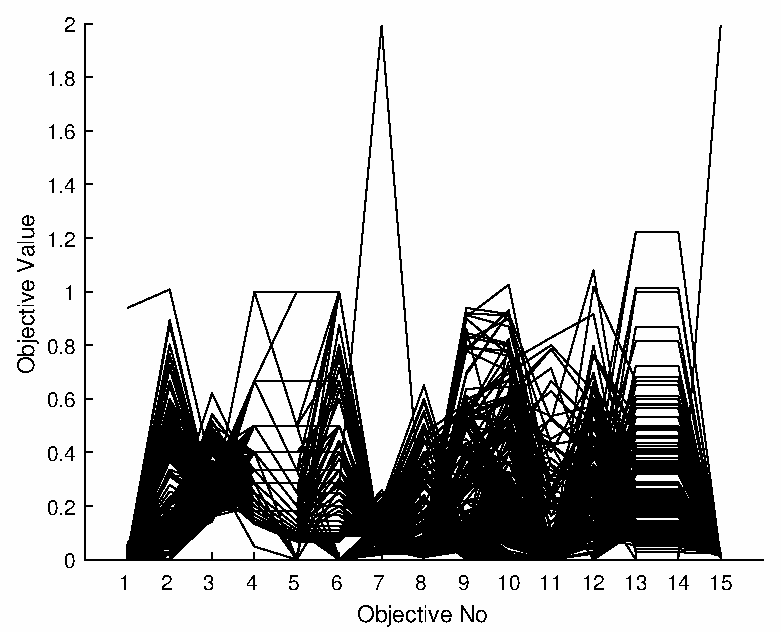
\includegraphics[width=0.4\textwidth]{pp/NSGAIII_15_19.eps}
	}
	\hspace{0em}	
	\subfigure[\textit{F}-NSGAIII]
	{
		\label{fig:dtlz710nsgaiiifigure}
		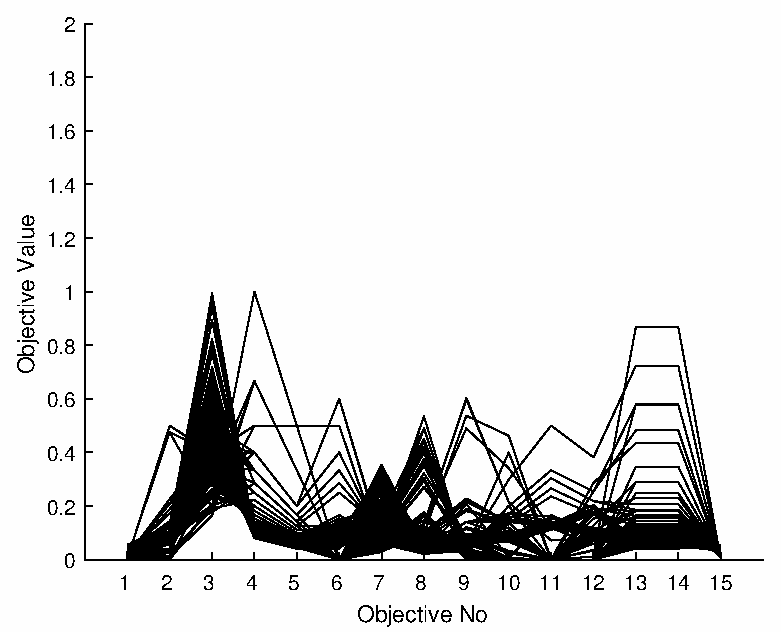
\includegraphics[width=0.4\textwidth]{pp/ENSGAIII_15_3.eps}
	}	
%	\hspace{0em}
%	\subfigure[MOEA/D]
%	{
%		\label{fig:dtlz710moeadfigure}
%		\includegraphics[width=0.170\textwidth]{figures/experiments/dtlz/moeaddtlz7_10.eps}
%	}	
%	\hspace{0em}	
%	\subfigure[FD-NSGAII]
%	{
%		\label{fig:dtlz710zhenanfigure}
%		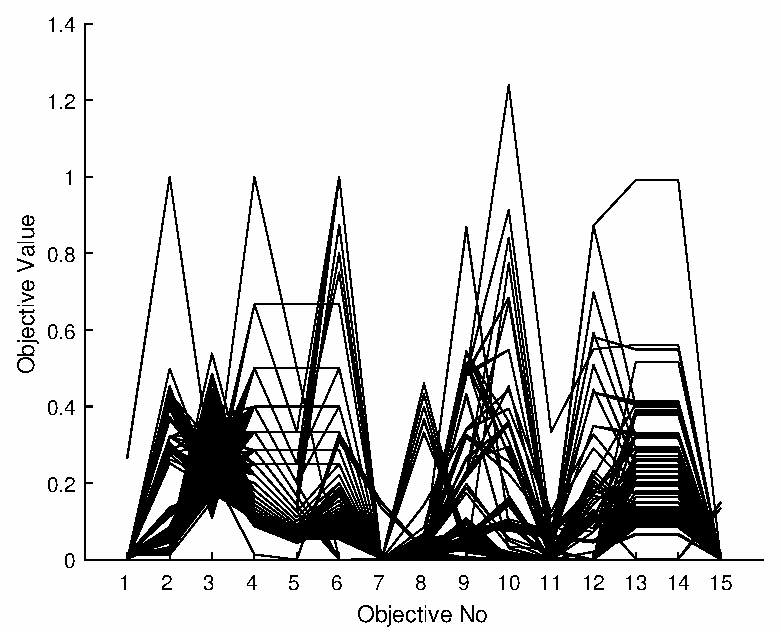
\includegraphics[width=0.170\textwidth]{pp/ical4j_ENSGAIII_15_1.eps}
%	}	
%	\hspace{0em}
%	\subfigure[HypE]
%	{
%		\label{fig:dtlz710hypefigure}
%		\includegraphics[width=0.170\textwidth]{figures/experiments/dtlz/hypedtlz7_10.eps}
%	}	
%	\hspace{0em}	
%	\subfigure[SDE]
%	{
%		\label{fig:dtlz710sdefigure}
%		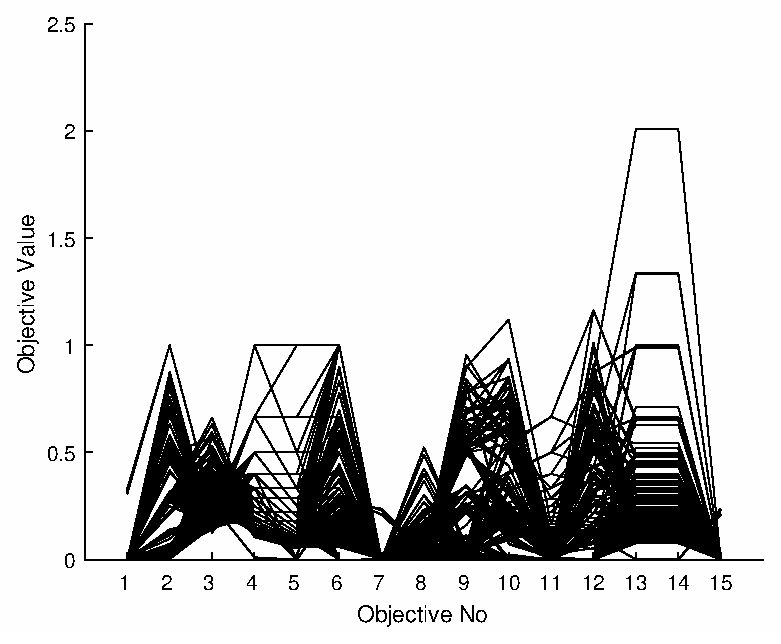
\includegraphics[width=0.170\textwidth]{pp/ical4j_NSGAIII_15_20.eps}
%	}	
%	\hspace{0em}
%	\subfigure[PICEAg]
%	{
%		\label{fig:dtlz710piceagfigure}
%		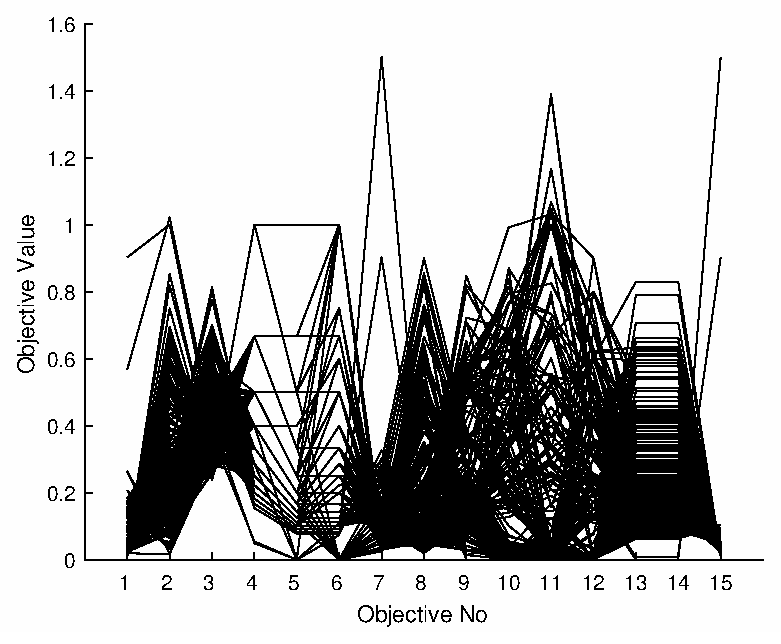
\includegraphics[width=0.170\textwidth]{pp/xapool_NSGAIII_15_20.eps}
%	}	
\caption{Parallel coordinate plot of all competing algorithms in $15-$ objective problem.}
\label{fig:dtlz710figure}
\end{figure*}


\begin{figure*}[h] 
\centering 
 
	\subfigure[NSGAIII]
	{
		\label{fig:dtlz710fdeafigure3d}
		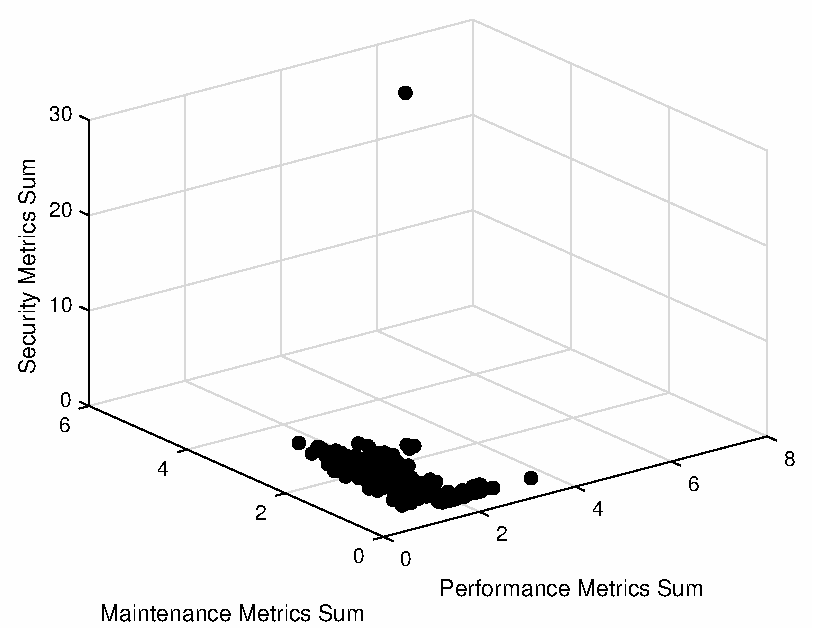
\includegraphics[width=0.4\textwidth]{3d/NSGAIII_15_15.eps}
	}
	\hspace{0em}	
	\subfigure[\textit{F}-NSGAIII]
	{
		\label{fig:dtlz710nsgaiiifigure3d}
		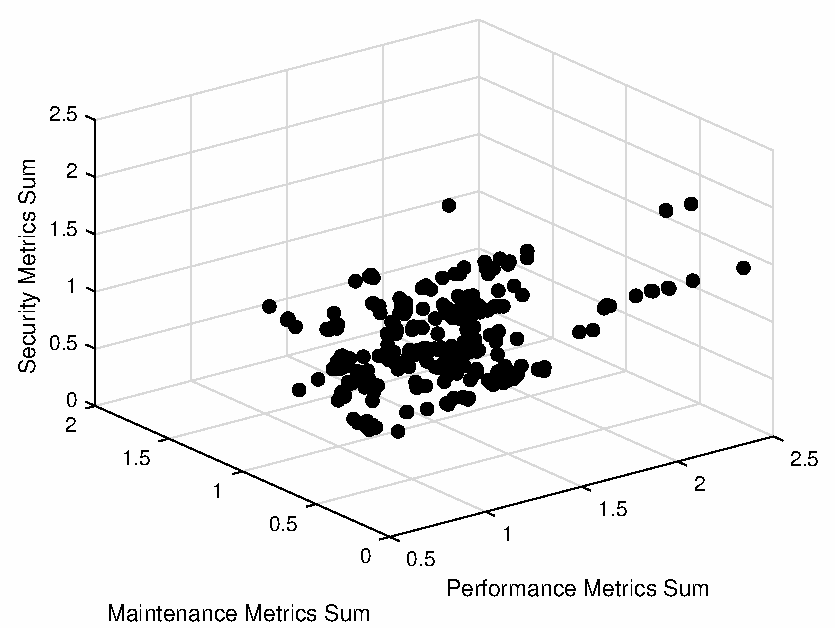
\includegraphics[width=0.4\textwidth]{3d/ENSGAIII_15_15.eps}
	}	
%	\hspace{0em}
%	\subfigure[MOEA/D]
%	{
%		\label{fig:dtlz710moeadfigure}
%		\includegraphics[width=0.170\textwidth]{figures/experiments/dtlz/moeaddtlz7_10.eps}
%	}	
%	\hspace{0em}	
%	\subfigure[FD-NSGAII]
%	{
%		\label{fig:dtlz710zhenanfigure}
%		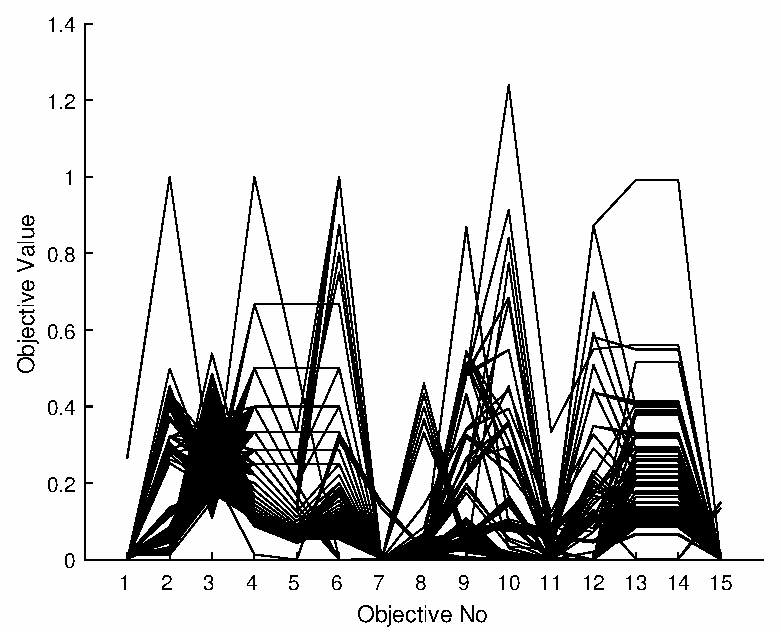
\includegraphics[width=0.170\textwidth]{pp/ical4j_ENSGAIII_15_1.eps}
%	}	
%	\hspace{0em}
%	\subfigure[HypE]
%	{
%		\label{fig:dtlz710hypefigure}
%		\includegraphics[width=0.170\textwidth]{figures/experiments/dtlz/hypedtlz7_10.eps}
%	}	
%	\hspace{0em}	
%	\subfigure[SDE]
%	{
%		\label{fig:dtlz710sdefigure}
%		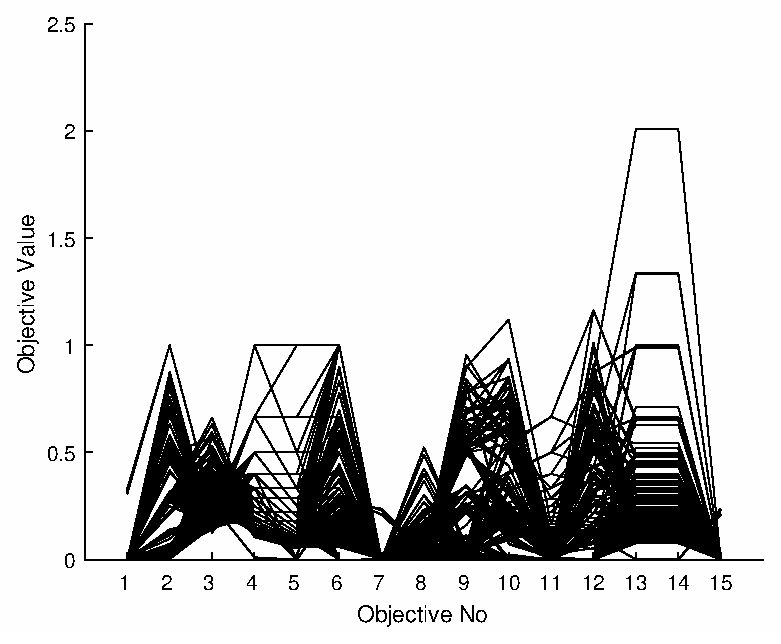
\includegraphics[width=0.170\textwidth]{pp/ical4j_NSGAIII_15_20.eps}
%	}	
%	\hspace{0em}
%	\subfigure[PICEAg]
%	{
%		\label{fig:dtlz710piceagfigure}
%		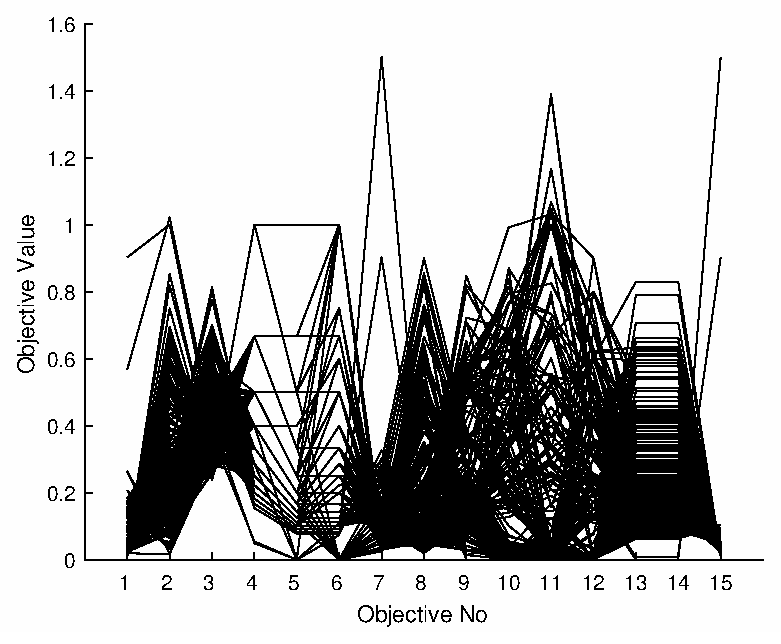
\includegraphics[width=0.170\textwidth]{pp/xapool_NSGAIII_15_20.eps}
%	}	
\caption{3D-plot of Metrics after converting 15 objective problems into 3 objective problem .}
\label{fig:dtlz710figure3d}
\end{figure*}



In our experiments, we have that seen in most cases \textit{F}-NSGAIII performs better than existing NSGAIII algorithms. 
On average, there are 6\% to 7\% improvements. But our proposed algorithms performs much better in big project with higher number of classes and higher number of relations. Here, Dependency relation type  does not affect the architecture much. But Aggregation, Composition, Association and Generalization relations are very important for software architecture.

\begin{itemize}
\item \textit{F}-NSGAIII performs much better in case high security concern i.e. with higher number of critical classes. In project \textit{sellwin} with very high number of critical classes, \textit{F}-NSGAIII achieves  17.566\% improvement.

\item \textit{F}-NSGAIII performs better with the increment of the complexity of the architecture. Here \textit{F}-NSGAIII performs  better  with higher number of relation ( in \textit{ical4j} 7.2111\%, and  in \textit{jspwiki} 7.206\%).

\item \textit{F}-NSGAIII does not get higher improvements in simpler architecture( \textit{jtidy} and \textit{java2html}).

\end{itemize}

% \begin{figure}  

\section{Discussion}
From experiment, it is acknowledged that \textit{F}-NSGAIII performs 
better than NSGAIII. The main reasons behind its better performance are:
We have incorporated domain knowledge by means of Gaussian functions. Now Gaussian functions are better to classify among two non dominated.
NSGAIII emphasizes on diversity, but some real world problems are hard to converge. Our aggregation gets advantages for convergence. This method is more effective for real world problems. 





% \label{fig:gaussian}
%   \includegraphics[width=\linewidth/2]{per_vs_rel.eps}
%   \caption{Performance vs Number of Relation}
% \end{figure}

% \begin{figure} 

% \label{fig:gaussian}
%   \includegraphics[width=\linewidth/2]{per_vs_cc.eps}
%   \caption{Performance vs Number of Critical Class}
% \end{figure}




\section{Conclusion}
In our work we tried to build up an automated process for finding the most suitable architecture of a software system. Here we have used 15 metrics to preciously evaluate the quality of the architecture. Among them there are 5 metrics related to security. In recent times, there are lots of work on search-based software architecture. But very few of them are related to security. Along with security, we also tried to optimize other metrics. As we have increased the number of objectives, we tried to develop a better algorithm to perform well with high number of objectives. Our modified algorithm performs better and have higher hyper-volume result. 

In our experiment, we gave all metrics same priority. In the real development process priority of different metrics may vary. We can change priority of different metrics multiplying weights with the normalized objectives. We plan to explore this in future and include more objectives from literature.



%\subsection{Software Architecture}
%These provided and received interfaces are linked by connectors. Through those connector, a component gets some services from another component. The functional requirements of the software are deeply depended on the the layout of the architecture.  So, this architecture is not only is the skeleton of the software system, but also a measurement tools of its performance, and other characteristics. This measurements are evaluated by experts opinion ~\cite{dobrica2002survey}. This architecture is followed through the entire process of the software architecture. But in the process of the software developments, there might be many modification in the requirements of the software. This modification imposes software developer to change basic parts of the software. Then for evaluation software with modification relies on the expertise of the software engineering.  These semi-automatic search base techniques can assist software developer to find the best alternatives of the original architecture. 

%In Ram{\'\i}ez et al.(\cite{ramirez2016comparative}), they formulate discovery of software architecture as a search problem. There UML class diagram of the software architecture is used as the information provider of the classes and relationship. Then a component is represented by a cohesive group of classes and there any classes must be belong to only one component \cite{ramirez2016comparative}. Two components are linked with connectors. Those connectors are the UML relation among the classes of that two connectors. Classes in the same component also might have relation with each other. According to UML 2, there are 5 types of relations :  associations, dependencies, aggregations, compositions and generalizations.






















































%\addtolength{\textheight}{-12cm}   % This command serves to balance the column lengths
                                  % on the last page of the document manually. It shortens
                                  % the textheight of the last page by auitable amount.
                                  % This command does not take effect until the next page
                                  % so it should come on the page before the last. Make
                                  % sure that you do not shorten the textheight too much.

%%%%%%%%%%%%%%%%%%%%%%%%%%%%%%%%%%%%%%%%%%%%%%%%%%%%%%%%%%%%%%%%%%%%%%%%%%%%%%%%



%%%%%%%%%%%%%%%%%%%%%%%%%%%%%%%%%%%%%%%%%%%%%%%%%%%%%%%%%%%%%%%%%%%%%%%%%%%%%%%%



%%%%%%%%%%%%%%%%%%%%%%%%%%%%%%%%%%%%%%%%%%%%%%%%%%%%%%%%%%%%%%%%%%%%%%%%%%%%%%%%
%\section*{APPENDIX}

%\section*{ACKNOWLEDGMENT}




%%%%%%%%%%%%%%%%%%%%%%%%%%%%%%%%%%%%%%%%%%%%%%%%%%%%%%%%%%%%%%%%%%%%%%%%%%%%%%%%




% Comment/uncomment as suits you
\bibliographystyle{ieeetr} %% IEEE transaction style
% \bibliographystyle{acm} %% ACM style
% \bibliographystyle{alpha}
\bibliography{ref}









\end{document}
